\documentclass[en,16:9,navbarinline,bigfoot]{sdqbeamer}
\usepackage[spanish]{babel}
\usepackage{booktabs}
\usepackage{rotating}

\titleimage{banner_2020_kit}

\groupname{Maestría en Ciencias de la Ingeniería Eléctrica}
\groupnamewidth{75mm}

\title[Problema de Investigación]{Trayectorias de Orden Superior Informadas por el Rendimiento de la Oblea}
\subtitle{Seminario I --- Problema de Investigación}
\author[R. Treviño]{Roberto Treviño Cervantes}
\newcommand{\shorttoday}{\ifnum\day<10 0\fi\number\day/\ifnum\month<10 0\fi\number\month/\number\year}
\date[\shorttoday]{\today}

\usepackage[citestyle=authoryear,bibstyle=numeric,hyperref,backend=biber,maxnames=1]{biblatex}
\addbibresource{presentation.bib}
\bibhang1em

\usepackage{tikz}
\usetikzlibrary{decorations.pathmorphing,patterns,arrows.meta,calc,positioning,3d,shapes.geometric,shapes.arrows,fit}
\usepackage{import}
\subimport{../../PlotNeuralNet/layers/}{init}

\def\ConvColor{rgb:yellow,5;red,2.5;white,5}
\def\ConvReluColor{rgb:yellow,5;red,5;white,5}
\def\PoolColor{rgb:red,1;black,0.3}
\def\UnpoolColor{rgb:blue,2;green,1;black,0.3}
\def\FcColor{rgb:blue,5;red,2.5;white,5}
\def\FcReluColor{rgb:blue,5;red,5;white,4}
\def\SoftmaxColor{rgb:magenta,5;black,7}

%%%%%%% ---- COLOR PALETTE --------
\definecolor{mnnwInk}     {HTML}{0A0A0A}
\definecolor{mnnwSignal}  {HTML}{0A84FF}
\definecolor{mnnwHair}    {HTML}{C9C9C9}
\definecolor{mnnwMute}    {HTML}{6F6F6F}
\definecolor{reticleFill} {HTML}{DCE6F7}
\definecolor{reticleEdge} {HTML}{4F6F9F}
\definecolor{reticleFlex} {HTML}{EEF3FB}
\definecolor{waferFill}   {HTML}{F5DCDC}
\definecolor{waferEdge}   {HTML}{9F4F4F}
\definecolor{waferFlex}   {HTML}{FBEEEE}
\definecolor{opticsFill}  {HTML}{E7DCF5}
\definecolor{opticsEdge}  {HTML}{6F4F9F}
\definecolor{opticsFlex}  {HTML}{F3EEFB}
\definecolor{frameFill}   {HTML}{D9E8D2}
\definecolor{frameEdge}   {HTML}{4F7F3F}
\definecolor{lensFill}    {HTML}{EEEEEE}

\tikzset{
  hdamper/.pic={
    \draw[line width=0.5pt, mnnwInk] (-0.45,0)            -- (-0.18,0);
    \draw[line width=0.5pt, mnnwInk] (-0.18,-0.11) rectangle (0.18,0.11);
    \draw[line width=0.5pt, mnnwInk] (0,-0.11)            -- (0,0.11);
    \draw[line width=0.5pt, mnnwInk] (0.18,0)             -- (0.45,0);
  },
  vdamper/.pic={
    \draw[line width=0.5pt, mnnwInk] (0,-0.45)            -- (0,-0.18);
    \draw[line width=0.5pt, mnnwInk] (-0.11,-0.18) rectangle (0.11,0.18);
    \draw[line width=0.5pt, mnnwInk] (-0.11,0)            -- (0.11,0);
    \draw[line width=0.5pt, mnnwInk] (0,0.18)             -- (0,0.45);
  },
}
\newcommand{\hdamperLong}[3]{%
  \pgfmathsetmacro{\xa}{#1}\pgfmathsetmacro{\xb}{#2}\pgfmathsetmacro{\yy}{#3}
  \pgfmathsetmacro{\Lcyl}{(\xb-\xa)*0.55}
  \pgfmathsetmacro{\xcylR}{\xa+\Lcyl}
  \pgfmathsetmacro{\xpisR}{\xb}
  \draw[line width=0.5pt, mnnwInk] (\xa,\yy-0.13) -- (\xa,\yy+0.13);
  \draw[line width=0.5pt, mnnwInk] (\xa,\yy+0.13) -- (\xcylR,\yy+0.13);
  \draw[line width=0.5pt, mnnwInk] (\xa,\yy-0.13) -- (\xcylR,\yy-0.13);
  \pgfmathsetmacro{\xpiston}{\xa+\Lcyl*0.70}
  \draw[line width=0.5pt, mnnwInk] (\xpiston,\yy-0.11) -- (\xpiston,\yy+0.11);
  \draw[line width=0.5pt, mnnwInk] (\xpiston,\yy) -- (\xpisR,\yy);
}
\newcommand{\vdamperLong}[3]{%
  \pgfmathsetmacro{\xx}{#1}\pgfmathsetmacro{\ya}{#2}\pgfmathsetmacro{\yb}{#3}
  \pgfmathsetmacro{\Lcyl}{(\yb-\ya)*0.55}
  \pgfmathsetmacro{\ycylT}{\ya+\Lcyl}
  \draw[line width=0.5pt, mnnwInk] (\xx-0.13,\ya) -- (\xx+0.13,\ya);
  \draw[line width=0.5pt, mnnwInk] (\xx-0.13,\ya) -- (\xx-0.13,\ycylT);
  \draw[line width=0.5pt, mnnwInk] (\xx+0.13,\ya) -- (\xx+0.13,\ycylT);
  \pgfmathsetmacro{\ypiston}{\ya+\Lcyl*0.70}
  \draw[line width=0.5pt, mnnwInk] (\xx-0.11,\ypiston) -- (\xx+0.11,\ypiston);
  \draw[line width=0.5pt, mnnwInk] (\xx,\ypiston) -- (\xx,\yb);
}

\def\getfirstchar#1#2\relax{#1}
\newcommand{\chainrow}[8]{%
  \edef\styleName{#2}%
  \def\currColor{mnnwMute}%
  \edef\firstChar{\expandafter\getfirstchar\styleName\relax}%
  \if\firstChar w\def\currColor{waferEdge}\fi
  \if\firstChar o\def\currColor{opticsEdge}\fi
  \if\firstChar r\def\currColor{reticleEdge}\fi
  \pgfmathparse{abs(#3 - \lastX) < 0.001 ? 1 : 0}
  \ifnum\pgfmathresult=1
    \pgfmathparse{abs(#3) < 0.001 ? 1 : 0}
    \ifnum\pgfmathresult=1 \def\lineColor{frameEdge} \else \def\lineColor{\currColor} \fi
    \draw[line width=0.35pt, \lineColor] (#3, \lastSpringY) -- (#3, #1-0.62);
  \fi
  \node[#2, inner xsep=6pt] (blk) at (#4,#1) {#5};
  \node[ghost, inner xsep=6pt] at (#3,#1) {\phantom{#5}};
  \draw[hsp] (#3, #1+0.62) -- (#4, #1+0.62);
  \draw[line width=0.35pt, mnnwInk] (#3, #1+0.275) -- (#3, #1+0.62);
  \draw[line width=0.35pt, mnnwInk] (#4, #1+0.275) -- (#4, #1+0.62);
  \draw[line width=0.35pt, mnnwInk] (#3, #1-0.275) -- (#3, #1-0.62);
  \draw[line width=0.35pt, mnnwInk] (#4, #1-0.275) -- (#4, #1-0.62);
  \hdamperLong{#3}{#4}{#1-0.62}
  \pgfmathsetmacro{\lblSide}{#4 > #3 ? #3 : #3}
  \pgfmathsetmacro{\lblAnch}{#4 > #3 ? "east" : "west"}
  \node[lbl, anchor=\lblAnch] at (\lblSide, #1+0.62) {#6};
  \node[lbl, anchor=\lblAnch] at (\lblSide, #1-0.62) {#7};
  \pgfmathsetmacro{\fSide}{#4 > #3 ? #4 : #4}
  \pgfmathsetmacro{\fAnch}{#4 > #3 ? "west" : "east"}
  \node[ftn, anchor=\fAnch] at (\fSide, #1-0.525) {#8};
  \draw[darr] (#3, #1-0.275) -- (#4, #1-0.275);
  \pgfmathsetmacro{\newSpringY}{#1+0.62}
  \xdef\lastSpringY{\newSpringY}
  \pgfmathsetmacro{\newX}{#4}
  \xdef\lastX{\newX}
}

%% Logo and Layout Settings
\kitlogo{uanl}
\grouplogo{fime}
\kitslogan{}

% Custom Title Frame Command to replace \KITtitleframe
\newcommand{\UANLtitleframe}{%
  \begin{frame}[plain]
    \begin{textblock*}{18mm}(7.3mm,6.7mm)
      
\includegraphics[width=18mm]{logos/uanl.eps}%
    \end{textblock*}%
    \begin{textblock*}{22mm}(\dimexpr\paperwidth-22.3mm\relax,6.7mm)
      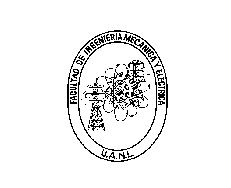
\includegraphics[width=22mm,height=22mm,keepaspectratio]{logos/fime.eps}%
    \end{textblock*}%
    \begin{textblock*}{\dimexpr\paperwidth-2\kitinnermargin\relax}[0,.5](7.3mm,35mm)
      {\usebeamerfont{title}\inserttitle}%
    \end{textblock*}%
    \begin{textblock*}{\dimexpr\paperwidth-2\kitinnermargin\relax}[0,.5](7.3mm,45mm)
      {\usebeamerfont{subtitle}\insertsubtitle}%
    \end{textblock*}%
    \begin{textblock*}{\dimexpr\paperwidth-2\kitinnermargin\relax}[0,.5](7.3mm,52mm)
      {\usebeamerfont{author}\insertauthor\ \textbar\ \insertdate}%
    \end{textblock*}%
    \begin{textblock*}{\paperwidth}(2mm,60mm)
      \centering
\includegraphics[height=30mm]{logos/banner_2020_kit.jpg}%
    \end{textblock*}%
  \end{frame}
}

\setbeamertemplate{frametitle}{%
  \begin{textblock*}{120mm}[0,1](7.3mm,15mm)
    {\usebeamerfont{frametitle}\insertframetitle}%
  \end{textblock*}%
  \begin{textblock*}{12mm}[1,1](\dimexpr\paperwidth-12.3mm\relax,15mm)
    
\includegraphics[width=8mm]{logos/uanl.eps}%
  \end{textblock*}%
  \begin{textblock*}{8mm}[1,1](\dimexpr\paperwidth-7.3mm\relax,15mm)
    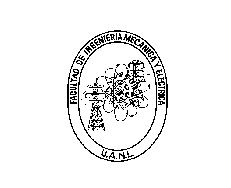
\includegraphics[width=10mm]{logos/fime.eps}%
  \end{textblock*}%
  \vspace{18mm}
}

\begin{document}

\UANLtitleframe

\begin{frame}{Índice}
\tableofcontents
\end{frame}

\section{Contexto}

\begin{frame}{Fotolitografía y la industria de los semiconductores}
    \begin{columns}
        \column{.6\textwidth}
        \begin{itemize}
          \item La fotolitografía (\textit{steppers} y \textit{scanners}) ha sido el sustento del avance tecnológico: ordenadores cada vez más capaces y modelos de IA cuya demanda computacional crece a pasos agigantados.
          \item Reducir el tamaño de los circuitos permite integrar más transistores por área con menor consumo: la dimensión crítica (CD) avanza hacia 18~nm en EUV mientras los dispositivos de consumo se fabrican a 38~nm en sistemas DUV.
          \item Es un proceso industrial de gran escala (millones de obleas/año sobre sustratos de 300~mm) en el que la exactitud nanométrica debe repetirse de forma continua.
        \end{itemize}
        \column{.4\textwidth}
        \centering
        \begin{tikzpicture}[scale=0.55, transform shape]
            \draw[fill=kit-yellow50, draw=mnnwInk] (-0.5, 5.0) rectangle (0.5, 4.6);
            \node[anchor=west, font=\tiny] at (0.6, 4.8) {Fuente de Luz};

            \draw[fill=reticleFill, draw=reticleEdge] (-1.8, 3.4) rectangle (1.8, 3.1);
            \draw[draw=kit-red100, -{Stealth[scale=1.2]}, line width=1.5pt] (1.2, 3.7) -- (-1.2, 3.7) node[left, font=\small\bfseries] {$\mathbf{v}_r$};
            \node[anchor=west, font=\tiny] at (1.9, 3.25) {Fotomáscara};

            \draw[fill=lensFill, draw=mnnwInk] (0, 1.8) ellipse (1.2cm and 0.25cm);
            \node[anchor=west, font=\tiny] at (1.3, 1.8) {Lente};

            \begin{scope}
                \clip (0, 0) ellipse (2.2cm and 0.45cm);
                \fill[waferFill] (-2.2, -0.45) rectangle (2.2, 0.45);
                \foreach \x in {-2.0,-1.75,...,2.0} {
                    \foreach \y in {-0.3, -0.15, 0, 0.15, 0.3} {
                        \draw[draw=waferEdge!40, line width=0.05pt] (\x-0.08, \y-0.06) rectangle (\x+0.08, \y+0.06);
                    }
                }
            \end{scope}
            \draw[fill=none, draw=waferEdge] (0, 0) ellipse (2.2cm and 0.45cm);
            \draw[draw=kit-blue100, -{Stealth[scale=1.2]}, line width=1.5pt] (-1.2, -0.75) -- (1.2, -0.75) node[right, font=\small\bfseries] {$\mathbf{v}_w$};
            \node[anchor=west, font=\tiny] at (2.3, 0) {Oblea};

            \draw[draw=mnnwSignal, line width=0.8pt, opacity=0.3] (0, 4.6) -- (0, 3.4);
            \draw[draw=mnnwSignal, line width=0.8pt, opacity=0.3] (0, 3.1) -- (0, 2.05);
            \draw[draw=mnnwSignal!80!black, line width=1.2pt, opacity=0.7] (0, 1.55) -- (0, 0.1);

            \begin{scope}[shift={(4.2, 3.5)}]
                \draw[draw=mnnwInk, fill=white] (-0.8,-1.2) rectangle (0.8,1.2);
                \fill[mnnwMute!40] (-0.8, 0.1) rectangle (0.8, 1.2);
                \foreach \h in {0.3, 0.6, 0.9} { \draw[mnnwInk, line width=1.2pt] (-0.5, \h) -- (0.5, \h); }
                \draw[draw=mnnwSignal, line width=0.8pt, dashed] (-0.9, -0.1) rectangle (0.9, 0.1);
                \node[anchor=south, font=\fontsize{3pt}{3pt}\selectfont, text=mnnwSignal] at (0, 0.1) {Slit};
                \draw[draw=mnnwInk, -Stealth, line width=1.2pt] (1.1, 0.5) -- (1.1, -0.5) node[midway, right, font=\fontsize{4pt}{4pt}\selectfont] {$\mathbf{v}$};
            \end{scope}
        \end{tikzpicture}
    \end{columns}
\end{frame}

\begin{frame}[fragile]{\textit{Step-and-Scan}: productividad bajo restricción de \textit{overlay}}
    \begin{columns}
        \column{.6\textwidth}
        \begin{itemize}
            \item En lugar de exponer la oblea completa, los scanners modernos realizan un barrido (\textit{scan}) en el que retícula y oblea se mueven sincronizadamente en direcciones opuestas (la retícula $4\times$ más rápido por la reducción del lente).
            \item La impresión de cada capa debe alinearse con las anteriores: un \textit{overlay} insuficiente vuelve inoperable al circuito y la oblea es desechada (\cite{Schmidt2012_UltraPrecision}).
            \item Se desplaza la oblea a gran velocidad para maximizar la productividad (\textit{throughput}), pero los perfiles de aceleración no deben comprometer el contraste ni la superposición exacta de las capas (\cite{Butler2011_PositionControl}).
        \end{itemize}
        \column{.4\textwidth}
        \begin{center}
          \resizebox{0.75\linewidth}{!}{
          \begin{tikzpicture}[
            every node/.style={font=\fontsize{4pt}{4pt}\selectfont},
            wafer/.style={draw=kit-blue100, line width=0.6pt, fill=kit-blue!5},
            die/.style={draw=mnnwInk, line width=0.3pt, fill=white, postaction={pattern=north east lines, pattern color=mnnwMute!40}},
            scan/.style={draw=kit-red100, line width=0.8pt, dashed, -{Stealth[scale=0.5]}},
            stepArrow/.style={draw=kit-lightgreen100, line width=0.8pt, -{Stealth[scale=0.5]}},
            traverse/.style={draw=mnnwInk, line width=0.5pt, dotted, -{Stealth[scale=0.5]}},
            point/.style={circle, fill=kit-blue100, inner sep=1pt}
          ]
            \draw[wafer] (0,0) circle (2.2cm);
            \begin{scope}
              \clip (0,0) circle (2.2cm);
              \foreach \x in {-1.75,-1.25,...,1.75} {
                \foreach \y in {-1.75,-1.25,...,1.75} {
                  \draw[die] (\x-0.2,\y-0.2) rectangle (\x+0.2,\y+0.2);
                }
              }
            \end{scope}
            \draw[scan] (-1.25, -1.75) -- (-1.25, -1.25);
            \draw[stepArrow] (-1.25, -1.25) -- (-0.75, -1.25);
            \draw[scan] (-0.75, -1.25) -- (-0.75, -1.75);
            \draw[stepArrow] (-0.75, -1.75) -- (-0.25, -1.75);
            \draw[scan] (-0.25, -1.75) -- (-0.25, -1.25);
            \draw[stepArrow] (-0.25, -1.25) -- (0.25, -1.25);
            \draw[scan] (0.25, -1.25) -- (0.25, -1.75);
            \draw[draw=mnnwInk, -Stealth] (0,0) -- (0.4,0) node[right] {$x$};
            \draw[draw=mnnwInk, -Stealth] (0,0) -- (0,0.4) node[above] {$y$};
          \end{tikzpicture}
          }
        \end{center}
    \end{columns}
\end{frame}

\begin{frame}{Vibraciones, tiempo de asentamiento y rendimiento (\textit{yield})}
    \begin{columns}
        \column{.55\textwidth}
        \begin{blueblock}{Overlay (nm)}
            Alineación entre las múltiples capas de un IC; condiciona directamente la operatividad del circuito (\cite{Schmidt2012_UltraPrecision}).
        \end{blueblock}

        \begin{greenblock}{Productividad (Obleas por Hora)}
            El alto costo de capital de las máquinas exige una producción rápida y continua.
        \end{greenblock}

        \vspace{0.2cm}
        El tiempo de asentamiento (\textit{settling time}) reduce la productividad pero mitiga las vibraciones residuales que degradan el \textit{overlay} (\cite{Butler2011_PositionControl}). Asumirlo como suficiente ignora la relación directa entre las vibraciones dinámicas y los \textbf{defectos espaciales} que determinan el rendimiento (\textit{yield}).

        \column{.45\textwidth}
        \centering
        \begin{tikzpicture}[scale=0.75, transform shape]
            \begin{scope}[shift={(0,3.5)}]
                \node[font=\tiny\bfseries, anchor=south] at (1.5, 2.5) {Vista Aérea};
                \foreach \i in {0,1} {
                    \foreach \j in {0,1} {
                        \begin{scope}[shift={(\i*1.8, \j*1.3)}]
                            \foreach \x in {0.1, 0.4, 0.7, 1.0} {
                                \draw[fill=kit-red100!60, draw=none] (\x, 0) rectangle (\x+0.2, 1);
                            }
                            \begin{scope}[shift={(0.12, 0)}]
                                \foreach \y in {0.1, 0.4, 0.7} {
                                    \draw[fill=kit-blue100!60, draw=none] (0, \y) rectangle (1.2, \y+0.2);
                                }
                            \end{scope}
                            \draw[draw=mnnwHair, dashed, line width=0.3pt] (0,0) rectangle (1.2, 1);
                        \end{scope}
                    }
                }
                \draw[draw=black, thick, dashed, rounded corners=1pt] (0, 1.3) rectangle (1.3, 2.3);
                \draw[draw=black, thick, dashed, rounded corners=1pt] (0, 0) rectangle (1.3, 1.0);
            \end{scope}
            \begin{scope}[shift={(0, 1.2)}]
                \draw[fill=kit-green100!80, draw=none] (0, 0) rectangle (2.5, 0.2);
                \draw[fill=kit-lightgreen100!30, draw=none] (0, 0.2) rectangle (2.5, 0.7);
                \foreach \x in {0.3, 0.8, 1.3, 1.8, 2.3} {
                     \draw[fill=kit-red100, draw=none] (\x-0.12, 0.2) rectangle (\x+0.12, 0.45);
                }
                \foreach \x in {0.45, 0.95, 1.45, 1.95, 2.45} {
                     \draw[fill=kit-blue100, draw=none] (\x-0.12, 0.7) rectangle (\x+0.12, 0.95);
                }
                \node[anchor=west, font=\fontsize{4pt}{4pt}\selectfont] at (2.6, 0.82) {Capa Actual};
                \node[anchor=west, font=\fontsize{4pt}{4pt}\selectfont] at (2.6, 0.32) {Capa Previa};
            \end{scope}
            \begin{scope}[shift={(0, -0.8)}]
                \draw[fill=kit-green100!80, draw=none] (0, 0) rectangle (2.5, 0.2);
                \draw[fill=kit-lightgreen100!30, draw=none] (0, 0.2) rectangle (2.5, 0.7);
                \foreach \x in {0.3, 0.8, 1.3, 1.8, 2.3} {
                     \draw[fill=kit-blue100, draw=none] (\x-0.12, 0.2) rectangle (\x+0.12, 0.45);
                }
                \foreach \x in {0.45, 0.95, 1.45, 1.95, 2.45} {
                     \draw[fill=kit-red100, draw=none] (\x-0.12, 0.7) rectangle (\x+0.12, 0.95);
                }
                \node[anchor=west, font=\fontsize{4pt}{4pt}\selectfont] at (2.6, 0.82) {Capa Actual};
                \node[anchor=west, font=\fontsize{4pt}{4pt}\selectfont] at (2.6, 0.32) {Capa Previa};
            \end{scope}
        \end{tikzpicture}
    \end{columns}
\end{frame}

\section{Identificación del vacío}

\begin{frame}{Estado del arte en control de movimiento}
    A escala nanométrica, los cuerpos del sistema \textbf{no} pueden tratarse como rígidos. La industria ha consolidado modelos variantes en el tiempo en los que las frecuencias naturales dependen de la posición instantánea del scanner.
    \vspace{0.2cm}
    \begin{itemize}
        \item \textbf{Control activo:} integradores no lineales (HIGS, CgLp) para mitigar el retraso de fase y reducir el sobretiro (\cite{Heertjes2025_NonlinearControl}).
        \item \textbf{Arquitecturas dinámicas:} configuración de triple etapa (\textit{fine stages}) (\cite{Al-Rawashdeh2022_Caracterization}).
        \item \textbf{\textit{Input shaping}:} trayectorias de referencia acotadas en el \textit{jerk}/\textit{snap} para evitar la excitación de modos resonantes (\cite{Al-Rawashdeh2023_Trajectories,Lambrechts2003_Trajectories}).
    \end{itemize}
    \vspace{0.2cm}
    Estos enfoques optimizan \textbf{métricas servo-mecánicas} (MSE, tiempo de asentamiento) y se mantienen aislados del proceso que pretenden controlar: la impresión del circuito integrado.
\end{frame}

\begin{frame}{La desconexión entre trayectoria y \textit{yield}}
    \begin{redblock}{Vacío identificado}
        La industria carece de una metodología que, de forma \textbf{predictiva}, traduzca los límites de la trayectoria $(v_{\max}, a_{\max}, j_{\max}, s_{\max})$ en la morfología del error sobre el patrón impreso.
    \end{redblock}
    \vspace{0.2cm}
    \begin{itemize}
        \item Existen múltiples patrones de vibración que producen \textbf{formas distintas} de error sobre la oblea; minimizar MSE no captura esa diferencia morfológica.
        \item Sin un modelo embebido en la planeación, se desconoce la correlación entre el perfil de movimiento y el impacto sobre la oblea.
        \item Esto obliga a usar parámetros conservadores y limita el avance de la \emph{manufactura reactiva} hacia una \emph{manufactura inteligente} consciente del contexto del proceso.
    \end{itemize}
\end{frame}

\section{Formulación del Problema}

\begin{frame}{Pregunta de investigación e hipótesis}
    \begin{purpleblock}{Pregunta}
        ¿En qué medida la integración de una \textbf{red neuronal convolucional} como modelo subrogado de predicción de defectos permite optimizar los parámetros cinemáticos de una \textbf{trayectoria de cuarto orden} para maximizar el rendimiento (\textit{yield}) sin penalizar la productividad (\textit{throughput}) del sistema?
    \end{purpleblock}

    \begin{blueblock}{Hipótesis}
        Es posible maximizar el \textit{yield} y la productividad de máquinas de litografía mediante perfiles de trayectoria de \textbf{15 segmentos (4to orden)} optimizados por un algoritmo bio-inspirado (\textbf{PSO}) que utiliza una CNN como métrica de evaluación de defectos.
    \end{blueblock}
\end{frame}

\begin{frame}{Variables del estudio}
    \begin{columns}
        \column{.5\textwidth}
        \textbf{Variables independientes}
        \begin{itemize}
            \item Tiempo de los segmentos de la trayectoria.
            \item Límites de los parámetros cinemáticos:
            \[ v_{\max},\; a_{\max},\; j_{\max},\; s_{\max} \]
        \end{itemize}
        \column{.5\textwidth}
        \textbf{Variables dependientes}
        \begin{itemize}
            \item Rendimiento de manufactura (\textit{yield}).
            \item Productividad (\textit{throughput}).
            \item Error de seguimiento dinámico.
        \end{itemize}
    \end{columns}
    \vspace{0.4cm}
    \begin{center}
    \small Las variables dependientes se combinan en una función de costo dinámica del tipo $T_{\text{ciclo}} \cdot (1 - \text{yield})$, que el optimizador minimiza.
    \end{center}
\end{frame}

\begin{frame}{Marco metodológico propuesto}
    \begin{center}
    \resizebox{0.95\linewidth}{!}{
    \begin{tikzpicture}[
        node distance=0.6cm,
        block/.style={rectangle, draw=mnnwInk, line width=0.4pt, rounded corners=2pt, minimum height=0.9cm, minimum width=2.0cm, align=center, font=\scriptsize},
        psoBlock/.style={block, fill=kit-yellow50!40},
        modBlock/.style={block, fill=reticleFill},
        yieldBlock/.style={block, fill=waferFill},
        dec/.style={diamond, draw=mnnwInk, line width=0.4pt, aspect=2.2, fill=kit-lightgreen100!20, font=\scriptsize, align=center, inner sep=1pt},
        grp/.style={draw=mnnwMute, dashed, line width=0.3pt, rounded corners=4pt, inner sep=6pt},
        flow/.style={-{Stealth[scale=0.9]}, line width=0.5pt, mnnwInk}
    ]
        \node[psoBlock] (pso) {Partículas\\$v_{\max}, a_{\max},$\\$j_{\max}, s_{\max}$};
        \node[dec, right=0.9cm of pso] (cost) {$T_{\text{ciclo}}\cdot(1-\text{yield})$};

        \node[modBlock, right=1.0cm of cost] (traj) {Generar\\trayectoria\\de alto orden};
        \node[modBlock, right=0.4cm of traj] (acc) {Calcular\\aceleración\\de referencia};
        \node[modBlock, right=0.4cm of acc] (mass) {Modelo\\masa-resorte\\de la plataforma};
        \node[modBlock, right=0.4cm of mass] (err) {Identificar\\errores como\\vibración};

        \node[yieldBlock, right=1.0cm of err] (map) {Construir\\mapa de\\defectos};
        \node[yieldBlock, right=0.4cm of map] (cls) {Detectar\\tipo de\\defectos (CNN)};

        \draw[flow] (pso) -- (cost);
        \draw[flow] (cost) -- (traj);
        \draw[flow] (traj) -- (acc);
        \draw[flow] (acc) -- (mass);
        \draw[flow] (mass) -- (err);
        \draw[flow] (err) -- (map);
        \draw[flow] (map) -- (cls);
        \draw[flow] (cls.north) -- ++(0,0.7) -| node[above, pos=0.25, font=\scriptsize] {Actualizar} (pso.north);

        \node[grp, fit={(pso) (cost)}, label={[font=\scriptsize\bfseries]above:Optimización (PSO)}] {};
        \node[grp, fit={(traj) (acc) (mass) (err)}, label={[font=\scriptsize\bfseries]above:Modelado (digital twin)}] {};
        \node[grp, fit={(map) (cls)}, label={[font=\scriptsize\bfseries]above:Estimación del rendimiento}] {};
    \end{tikzpicture}
    }
    \end{center}
    \vspace{0.1cm}
    \scriptsize El algoritmo bio-inspirado \textbf{PSO} explora el espacio de parámetros; cada propuesta atraviesa el \emph{digital twin} y el clasificador CNN, devolviendo un costo que combina productividad y rendimiento.
\end{frame}

\section{Delimitación}

\begin{frame}[fragile]{Modelo dinámico de cadena flexible}
        \begin{center}
          \begin{turn}{90}
          \resizebox{0.39\linewidth}{!}{
          \begin{tikzpicture}[scale=1, transform shape,
            every node/.style    ={font=\small},
            rfrm/.style          ={draw=frameEdge, line width=0.6pt, fill=frameFill, minimum height=0.80cm, font=\small\bfseries, inner sep=2pt},
            rblk/.style          ={draw=reticleEdge, line width=0.5pt, fill=reticleFill, minimum height=0.55cm, font=\footnotesize, text=mnnwInk, inner sep=2.5pt},
            rflx/.style          ={draw=reticleEdge, line width=0.4pt, fill=reticleFlex, minimum height=0.42cm, font=\scriptsize, text=mnnwInk, inner sep=2pt, dashed},
            wblk/.style          ={draw=waferEdge, line width=0.5pt, fill=waferFill, minimum height=0.55cm, font=\footnotesize, text=mnnwInk, inner sep=2.5pt},
            wflx/.style          ={draw=waferEdge, line width=0.4pt, fill=waferFlex, minimum height=0.42cm, font=\scriptsize, text=mnnwInk, inner sep=2pt, dashed},
            oblk/.style          ={draw=opticsEdge, line width=0.5pt, fill=opticsFill, minimum height=0.55cm, font=\footnotesize, text=mnnwInk, inner sep=2.5pt},
            oflx/.style          ={draw=opticsEdge, line width=0.4pt, fill=opticsFlex, minimum height=0.42cm, font=\scriptsize, text=mnnwInk, inner sep=2pt, dashed},
            ghost/.style         ={draw=mnnwHair, dashed, line width=0.35pt, fill=none, minimum height=0.55cm},
            hsp/.style           ={line width=0.5pt, mnnwInk, decorate, decoration={zigzag, segment length=3.6pt, amplitude=2pt, pre length=2pt, post length=2pt}},
            vsp/.style           ={line width=0.5pt, mnnwInk, decorate, decoration={zigzag, segment length=3.6pt, amplitude=2pt, pre length=2pt, post length=2pt}},
            darr/.style          ={Stealth-Stealth, line width=0.5pt, mnnwSignal},
            lbl/.style           ={font=\scriptsize, text=mnnwInk},
            ftn/.style           ={font=\scriptsize, text=mnnwSignal},
            axis/.style          ={dashed, line width=0.4pt, mnnwMute},
            pillar/.style        ={fill=black!8, draw=mnnwHair, line width=0.3pt},
            hatchfloor/.style    ={pattern=north east lines, pattern color=mnnwMute},
          ]
          \def\xLeft{-8.0}\def\xRight{8.0}
          \def\xPilL{-7.4}\def\xPilR{7.4}
          \def\yFloor{0}
          \def\yBase{1.4}
          \def\yWa{3.4}\def\yWb{5.4}\def\yWc{7.4}\def\yWd{9.4}\def\yWe{11.4}\def\yWf{13.4}
          \def\yOa{17.2}\def\yOb{19.2}\def\yOc{21.2}
          \def\yRa{25.2}\def\yRb{27.2}\def\yRc{29.2}\def\yRd{31.2}\def\yRe{33.2}\def\yRf{35.2}
          \def\yTop{35.5}
          \def\yShA{15.4}\def\yShB{23.2}
          \filldraw[hatchfloor, draw=mnnwInk, line width=0.7pt]
            (\xRight, 0) -- (\xLeft-0.6, 0) -- (\xLeft-0.6, \yWb) -- (\xLeft-1.1, \yWb)
            -- (\xLeft-1.1, -0.5) -- (\xRight, -0.5) -- cycle;
          \node[lbl, anchor=west] at (\xRight+0.08,0.20) {$\mathcal{F}_0$};
          \draw[axis] (0,-0.05) -- (0,\yTop);
          \filldraw[draw=frameEdge, line width=0.6pt, fill=frameFill]
            (7.8, \yBase-0.4) -- (-7.8, \yBase-0.4) -- (-7.8, \yTop) -- (-7.4, \yTop)
            -- (-7.4, \yShB+0.4) -- (7.8, \yShB+0.4) -- (7.8, \yShB-0.4) -- (-7.4, \yShB-0.4)
            -- (-7.4, \yShA+0.4) -- (7.8, \yShA+0.4) -- (7.8, \yShA-0.4) -- (-7.4, \yShA-0.4)
            -- (-7.4, \yBase+0.4) -- (7.8, \yBase+0.4) -- cycle;
          \node[font=\small\bfseries, text=mnnwInk] at (0, \yBase) {Marco Base $\;(\mathcal{F}_1)$};
          \hdamperLong{\xLeft-0.6}{-7.8}{2.5}
          \node[lbl, above=2pt] at ({(\xLeft-0.6-7.8)/2}, 2.5) {$C_1$};
          \draw[hsp] (\xLeft-0.6, 2.0) -- (-7.8, 2.0) node[midway, below=4pt, lbl] {$K_1$};
          \pgfmathsetmacro{\shelfW}{\yBase+0.4}
          \xdef\lastSpringY{\shelfW} \xdef\lastX{0}
          \chainrow{\yWa}{wblk}{0}{ 0.9}{\textbf{Oblea LS} $(i_3{=}2)$}{$K_{2,3}$}{$C_{2,3}$}{$f_{2,3}$}
          \chainrow{\yWb}{wflx}{0.9}{ 1.8}{Acoplamiento flexible $(i_3{=}3)$}{$K_{3,3}$}{$C_{3,3}$}{$f_{3,3}$}
          \chainrow{\yWc}{wblk}{1.8}{ 2.7}{\textbf{Oblea SS} $(i_3{=}4)$}{$K_{4,3}$}{$C_{4,3}$}{$f_{4,3}$}
          \chainrow{\yWd}{wflx}{2.7}{ 3.6}{Acoplamiento flexible $(i_3{=}5)$}{$K_{5,3}$}{$C_{5,3}$}{$f_{5,3}$}
          \chainrow{\yWe}{wblk}{3.6}{ 4.5}{\textbf{Plataforma de la Oblea} $(i_3{=}6)$}{$K_{6,3}$}{$C_{6,3}$}{$f_{6,3}$}
          \chainrow{\yWf}{wblk}{4.5}{ 5.4}{\textbf{Dado} $(N_3{=}7)$}{$K_{N_3,3}$}{$C_{N_3,3}$}{$f_{N_3,3}$}
          \pgfmathsetmacro{\shelfO}{\yShA+0.4}
          \xdef\lastSpringY{\shelfO} \xdef\lastX{0}
          \chainrow{\yOa}{oblk}{0}{-0.9}{\textbf{Marco de Metrología} $(i_2{=}2)$}{$K_{2,2}$}{$C_{2,2}$}{$f_{2,2}$}
          \chainrow{\yOb}{oblk}{-0.9}{-1.8}{Caja de Óptica $(i_2{=}3)$}{$K_{3,2}$}{$C_{3,2}$}{$f_{3,2}$}
          \chainrow{\yOc}{oblk}{-1.8}{-2.7}{Lente $(i_2{=}4)$}{$K_{4,2}$}{$C_{4,2}$}{$f_{4,2}$}
          \pgfmathsetmacro{\shelfR}{\yShB+0.4}
          \xdef\lastSpringY{\shelfR} \xdef\lastX{0}
          \chainrow{\yRa}{rblk}{0}{-0.9}{\textbf{Retícula LS} $(i_1{=}2)$}{$K_{2,1}$}{$C_{2,1}$}{$f_{2,1}$}
          \chainrow{\yRb}{rflx}{-0.9}{-1.8}{Acoplamiento flexible $(i_1{=}3)$}{$K_{3,1}$}{$C_{3,1}$}{$f_{3,1}$}
          \chainrow{\yRc}{rblk}{-1.8}{-2.7}{\textbf{Retícula SS} $(i_1{=}4)$}{$K_{4,1}$}{$C_{4,1}$}{$f_{4,1}$}
          \chainrow{\yRd}{rflx}{-2.7}{-3.6}{Acoplamiento flexible $(i_1{=}5)$}{$K_{5,1}$}{$C_{5,1}$}{$f_{5,1}$}
          \chainrow{\yRe}{rblk}{-3.6}{-4.5}{\textbf{Plataforma de la Retícula} $(i_1{=}6)$}{$K_{6,1}$}{$C_{6,1}$}{$f_{6,1}$}
          \chainrow{\yRf}{rblk}{-4.5}{-5.4}{\textbf{Fotomáscara} $(N_1{=}7)$}{$K_{N_1,1}$}{$C_{N_1,1}$}{$f_{N_1,1}$}
          \draw[line width=0.4pt, waferEdge]   (\xPilR+0.30,\yWa-0.30) -- (\xPilR+0.30,\yWf+0.30);
          \node[font=\scriptsize\bfseries, text=waferEdge, rotate=-90, anchor=south] at (\xPilR+0.55,{(\yWa+\yWf)/2}) {Cadena de la oblea $(j{=}3)$};
          \draw[line width=0.4pt, opticsEdge]  (\xPilR+0.30,\yOa-0.30) -- (\xPilR+0.30,\yOc+0.30);
          \node[font=\scriptsize\bfseries, text=opticsEdge, rotate=-90, anchor=south] at (\xPilR+0.55,{(\yOa+\yOc)/2}) {Cadena de óptica $(j{=}2)$};
          \draw[line width=0.4pt, reticleEdge] (\xPilR+0.30,\yRa-0.30) -- (\xPilR+0.30,\yRf+0.30);
          \node[font=\scriptsize\bfseries, text=reticleEdge, rotate=-90, anchor=south] at (\xPilR+0.55,{(\yRa+\yRf)/2}) {Cadena de la retícula $(j{=}1)$};
          \end{tikzpicture}
          }
          \end{turn}
        \end{center}
\end{frame}

\begin{frame}{Dinámica planar: $X$, $Y$, $\theta_z$}
    \begin{itemize}
        \item Adoptamos el modelo multicuerpo flexible de \cite{Al-Rawashdeh2022_Caracterization}: retícula, óptica y oblea forman \textbf{tres cadenas seriales} acopladas al marco base.
        \item Limitamos el movimiento a los desplazamientos planares $f_{i_{j_x}}$, $f_{i_{j_y}}$ y la \textbf{rotación planar} $\theta_z$. Se ignora $Z$ (sólo se usa previo a la exposición para alinear la fotomáscara).
        \item Consideramos 16 cuerpos ($N_1=6$, $N_2=3$, $N_3=6$) que requieren 6 estados para su descripción:
        \begin{equation*}
            x =
            \begin{bmatrix}
                \underbrace{x_1, \ldots, x_6}_{\text{marco base}} \;,\;
                \underbrace{x_7, \ldots, x_{6N_1}}_{\text{cadena 1}} \;,\;
                \underbrace{\ldots}_{\text{cadena 2}} \;,\;
                \underbrace{\ldots}_{\text{cadena 3}}
            \end{bmatrix}^T
        \end{equation*}
        \item Para un cuerpo $2 < i < N_j$:
        \begin{align*}
            \ddot{\mathbf{x}}_{2p-1} &= \tfrac{1}{\bar{m}_{i_j}}\big[u^0_{i_j} - {}^0\bar{C}_{i_j}\dot{\mathbf{x}}_{2p-1} - {}^0\bar{K}_{i_j}\mathbf{x}_{2p-1} + {}^0\hat{C}_{(i+1)_j}\dot{\mathbf{x}}_{2p+1} + {}^0\hat{K}_{(i+1)_j}\mathbf{x}_{2p+1}\big] \\
            &\quad - \tfrac{1}{\bar{m}_{(i-1)_j}}\big[u^0_{(i-1)_j} - {}^0\bar{C}_{(i-1)_j}\dot{\mathbf{x}}_{2p-3} - {}^0\bar{K}_{(i-1)_j}\mathbf{x}_{2p-3} + {}^0\hat{C}_{i_j}\dot{\mathbf{x}}_{2p-1} + {}^0\hat{K}_{i_j}\mathbf{x}_{2p-1}\big]
        \end{align*}
    \end{itemize}
\end{frame}

\begin{frame}{Simulación: \textit{digital twin} en MuJoCo}
    \begin{columns}
        \column{.6\textwidth}
        \begin{itemize}
            \item Implementación del modelo multicuerpo en \textbf{MuJoCo} (\cite{todorov2012mujoco}), usando los parámetros propuestos en \cite{Al-Rawashdeh2022_Caracterization}.
            \item Permite generar \emph{mapas de defectos} a partir del error de seguimiento de una trayectoria con ciertos parámetros dinámicos.
            \item Es la única vía de validación: no se cuenta con un scanner litográfico físico (alto costo y complejidad).
        \end{itemize}
        \begin{center}
          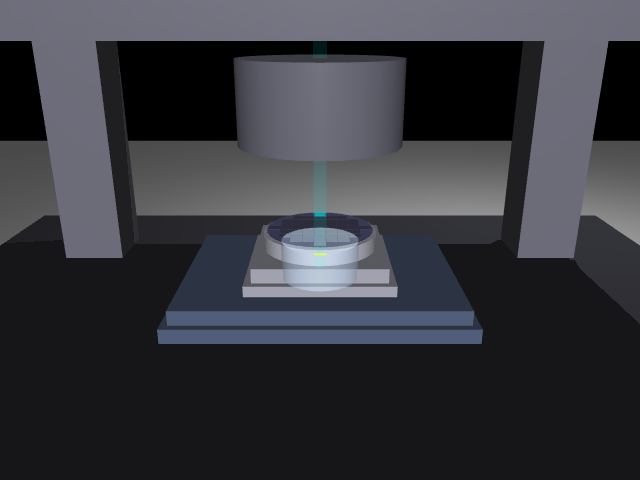
\includegraphics[width=0.4\linewidth]{pictures/scanning_3d.png}
        \end{center}
        \column{.4\textwidth}
        \begin{center}
          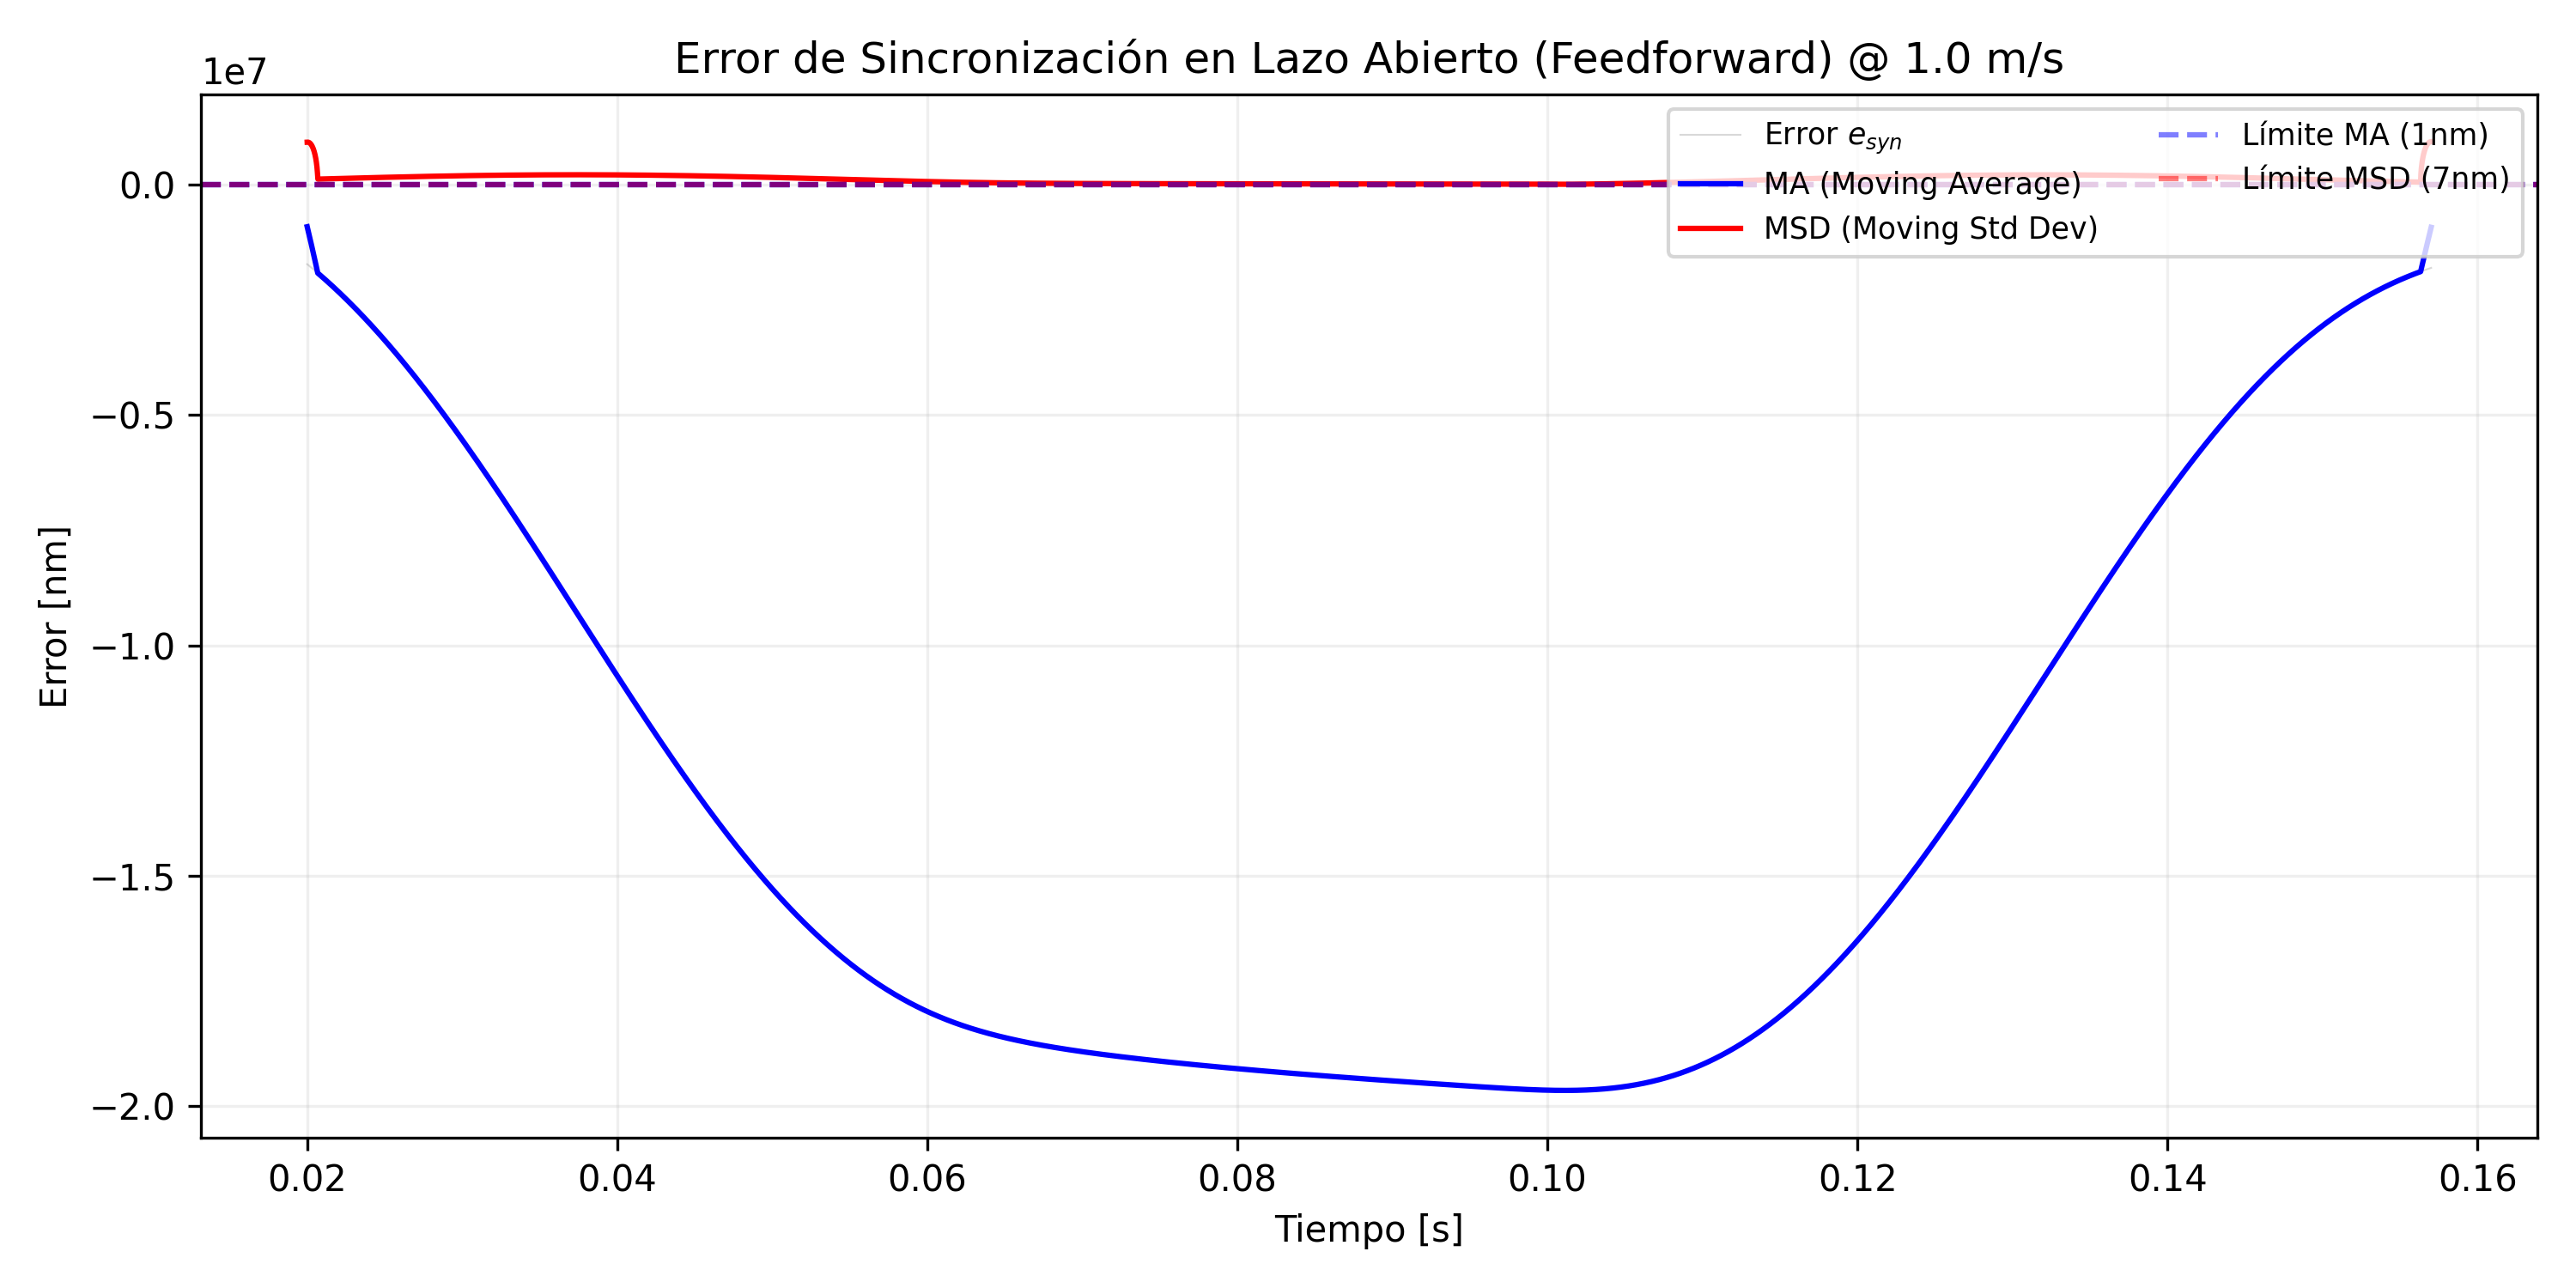
\includegraphics[width=\linewidth]{pictures/sim_graph_ff.png}
        \end{center}
    \end{columns}
\end{frame}

\begin{frame}{Datos y CNN como modelo subrogado}
    \begin{columns}[T]
        \column{.55\textwidth}
        \begin{itemize}
            \item Conjunto de datos \textbf{WM-811K} con 811{,}457 mapas de defectos de manufactura real (\cite{Wu2015_WM811K}).
            \item Subconjunto de 172{,}950 muestras etiquetadas en 9 clases (\textit{Center}, \textit{Edge-Loc}, \textit{Scratch}, \textit{Donut}, \ldots).
            \item Entrenamiento sobre cómputo rentado en \textbf{AWS g4dn.xlarge}.
            \item La CNN actúa como \textbf{función de costo dinámica} sobre los mapas que produce el \textit{digital twin}.
        \end{itemize}
        \column{.45\textwidth}
        \begin{center}
          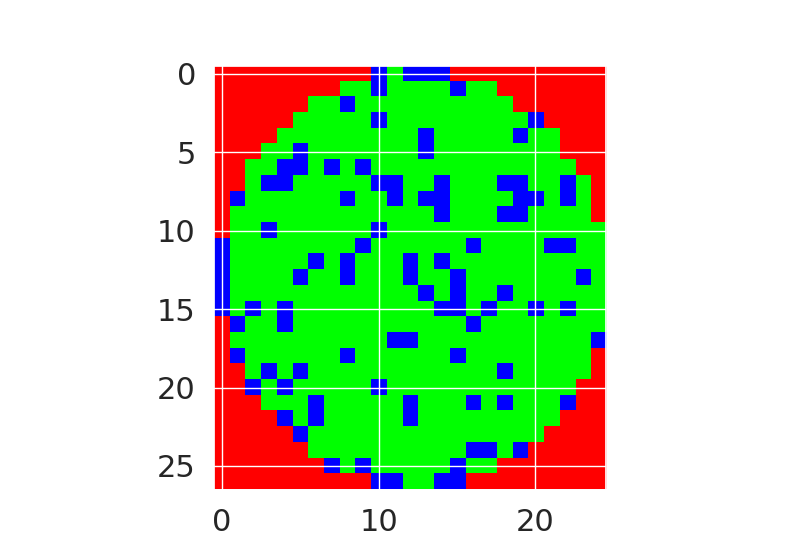
\includegraphics[width=0.7\linewidth]{pictures/mapa.png}
        \end{center}
    \end{columns}

    \vspace{0.15cm}
    \centering
    \scriptsize
    \begin{tabular}{ll@{\hspace{0.6cm}}ll}
        \toprule
        \textbf{Parámetro} & \textbf{Valor} & \textbf{Parámetro} & \textbf{Valor} \\
        \midrule
        Entrada & $64 \times 64$ & Optimización & Adam ($\text{lr}=10^{-3}$), 5 Epochs \\
        Arquitectura & 3$\times$Conv, 2$\times$FC (16, 32, 64) & \textbf{Precisión} & \textbf{96.88\%} \\
        Pérdida & CrossEntropy & Validación & Mapas simulados (MuJoCo) \\
        \bottomrule
    \end{tabular}
\end{frame}

\begin{frame}{Trayectorias de cuarto orden (15 segmentos)}
    \begin{columns}
        \column{.58\textwidth}
        \begin{itemize}
            \item Trayectorias de referencia con derivadas de orden superior acotadas (\textit{snap} finito), construidas como polinomios segmentados óptimos en tiempo (\cite{Lambrechts2003_Trajectories}).
            \item Perfiles de \textbf{15 segmentos} derivados analíticamente con \textit{input shaping} (\cite{Al-Rawashdeh2023_Trajectories}).
            \item Sus parámetros $(v_{\max}, a_{\max}, j_{\max}, s_{\max})$ y los tiempos de segmento son las entradas que PSO optimiza.
        \end{itemize}
        \column{.42\textwidth}
        \begin{center}
          \resizebox{0.88\linewidth}{!}{
          \begin{tikzpicture}[
            every node/.style={font=\fontsize{4pt}{4pt}\selectfont},
            wafer/.style={draw=kit-blue100, line width=0.6pt, fill=kit-blue!5},
            die/.style={draw=mnnwInk, line width=0.3pt, fill=white, postaction={pattern=north east lines, pattern color=mnnwMute!40}},
            square/.style={draw=mnnwInk, line width=0.8pt},
            fillet/.style={draw=mnnwSignal, line width=0.8pt},
            meander/.style={draw=opticsEdge, line width=0.8pt},
            axis/.style={draw=mnnwInk, -Stealth}
          ]
            \draw[wafer] (0,0) circle (2.2cm);
            \begin{scope}
              \clip (0,0) circle (2.2cm);
              \foreach \x in {-1.75,-1.25,...,1.75} {
                \foreach \y in {-1.75,-1.25,...,1.75} {
                  \draw[die] (\x-0.2,\y-0.2) rectangle (\x+0.2,\y+0.2);
                }
              }
            \end{scope}
            \draw[mnnwInk, line width=0.8pt, dashed] (-1.25, -1.75) -- (-1.25, -1.25);
            \draw[square] (-1.25, -1.25) -- (-1.25, -1.0) -- (-0.75, -1.0) -- (-0.75, -1.25);
            \draw[fillet] (-1.25, -1.25) -- (-1.25, -1.12)
                          arc(180:90:0.12) -- (-0.87, -1.0)
                          arc(90:0:0.12) -- (-0.75, -1.12)
                          -- (-0.75, -1.25);
            \draw[meander] (-1.25, -1.25) to[out=90, in=180] (-1.0, -1.0) to[out=0, in=90] (-0.75, -1.25);
            \draw[mnnwInk, line width=0.8pt, dashed] (-0.75, -1.25) -- (-0.75, -1.75);
            \begin{scope}[shift={(0.25, 1.35)}]
              \draw[square]  (0, 0.55) -- (0.35, 0.55) node[right, font=\fontsize{3.5pt}{3.5pt}\selectfont] {Cuadrado};
              \draw[fillet]  (0, 0.27) -- (0.35, 0.27) node[right, font=\fontsize{3.5pt}{3.5pt}\selectfont] {Bisel};
              \draw[meander] (0, 0.00) -- (0.35, 0.00) node[right, font=\fontsize{3.5pt}{3.5pt}\selectfont] {Meandro};
            \end{scope}
            \draw[axis] (0,0) -- (0.4,0) node[right] {$x$};
            \draw[axis] (0,0) -- (0,0.4) node[above] {$y$};
          \end{tikzpicture}
          }
        \end{center}
    \end{columns}
\end{frame}

\begin{frame}{Alcances, exclusiones y riesgos}
    \begin{columns}
        \column{.5\textwidth}
        \textbf{Dentro del alcance}
        \begin{itemize}
            \item Modelado dinámico de cadena flexible planar ($X$, $Y$, $\theta_z$).
            \item Generación analítica de trayectorias acotadas en \textit{snap}.
            \item Entrenamiento de CNN sobre WM-811K.
            \item Optimización con PSO usando la CNN como costo.
        \end{itemize}
        \column{.5\textwidth}
        \textbf{Fuera del alcance}
        \begin{itemize}
            \item Implementación en hardware real.
            \item Diseño óptico del sistema litográfico.
            \item Compensación de efectos térmicos.
            \item Movimiento en el eje $Z$.
        \end{itemize}
    \end{columns}
    \vspace{0.25cm}
    \begin{redblock}{Riesgo principal}
        La complejidad de la función de costo dinámica (modelo multicuerpo de \cite{Al-Rawashdeh2022_Caracterization} acoplado a la CNN) puede degradar los tiempos de convergencia del algoritmo PSO.
    \end{redblock}
\end{frame}

\section{Línea de Generación y Aplicación del Conocimiento}

\begin{frame}{LGAC: Tecnología e Innovación Mecatrónica}
    \begin{purpleblock}{Adscripción}
        El estudio se inscribe en la línea \textbf{Tecnología e Innovación Mecatrónica}, al involucrar \emph{sistemas inteligentes} para resolver problemas de \emph{control de movimiento} en sistemas industriales.
    \end{purpleblock}
    \vspace{0.2cm}
    \begin{itemize}
        \item Aporta una metodología \emph{predictiva} que conecta planeación de trayectorias y rendimiento (\textit{yield}).
        \item Habilita explorar perfiles de aceleración más agresivos sin incurrir en mermas masivas.
        \item Es un estudio de tipo \emph{metodológico y computacional}: el resultado es un \emph{framework} de simulación y optimización para la prevención de fallas.
    \end{itemize}
    \vspace{0.4cm}
    \begin{center}
    \textit{Gracias por su atención.}
    \end{center}
\end{frame}

\appendix
\beginbackup
\begin{frame}[allowframebreaks]{Referencias}
\printbibliography
\end{frame}
\backupend

\end{document}
